% ==========================================
% LatexRefinement Step Output: step4-03-31-25-tuesday-all-offset-final.tex
% Model: gemini-3.5-flash
% Temperature: 0.33
% TopP: 0.95
% TopK: 40
% MaxOutputTokens: 65535
% ThinkingBudget: 32765
% ThinkingLevel: HIGH
% Prompt Tokens: 48'834
% Candidates Tokens: 22'547 (inkl. Thinking Tokens)
% Cached Tokens: 0
% Processed on: 2026-07-18 18:14:12
% ==========================================

\lecturechapter{Dienstag}{31. Mär}{31. März 2025}{Das Auswahlaxiom, das Banach-Tarski-Paradoxon und das Lemma von Zorn}
% Old chapter title: Das Auswahlaxiom und das Banach-Tarski-Paradoxon

\begin{nice-box}[Vorlesungsübersicht \& Kontext]
In dieser Vorlesung führt Dr. Fabian Ziltener (in Vertretung für Christian Urech) das fundamentale \newterm{Auswahlaxiom} ($\text{AC}$) ein. Neben der anschaulichen Motivation durch das berühmte \newterm{Banach-Tarski-Paradoxon} erarbeiten wir die formalen Grundlagen und äquivalenten Formulierungen dieses zentralen Axioms der Mengenlehre.

Die Themenschwerpunkte dieser Vorlesung umfassen:
\begin{itemize}
    \item \textbf{Das Banach-Tarski-Paradoxon:} Eine kontraintuitive, aber mathematisch exakte Konsequenz des Auswahlaxioms in der dreidimensionalen Geometrie.
    \item \textbf{Äquivalente Formulierungen des Auswahlaxioms:} Die Definition über Auswahlfunktionen ($\text{AC}$) und die Formulierung über das allgemeine kartesische Produkt ($\text{AC}'$).
    \item \textbf{Das Wohlordnungsprinzip ($\text{WOP}$):} Die Aussage, dass jede Menge wohlgeordnet werden kann, und der Beweis der Äquivalenz $\text{AC} \leftrightarrow \text{WOP}$ unter Verwendung von \newterm{Ordinalzahlen}.
    \item \textbf{Das Kuratowski-Zornsche Lemma ($\text{KZL}$):} Das unentbehrliche Werkzeug der mathematischen Praxis zur Existenz maximaler Elemente in halbgeordneten Mengen.
\end{itemize}
\end{nice-box}

\section{Das Banach-Tarski-Paradoxon}

\begin{spoken-clean}[00:00:00 - 00:01:46]
Ah, jetzt. Guten Tag. Mein Name ist Fabian Ziltener, ich vertrete Christian Urech heute für diese Vorlesung über Grundstrukturen und möchte mit einem Video anfangen. Und dann sehen wir, was das mit Grundstrukturen zu tun hat. Also hier ist es, ich hoffe, dass Sie etwas hören. Vielleicht muss ich das Mikrofon dann hinhalten, aber mal schauen.

\inlinemetanote{Ein Video von Vsauce über das Banach-Tarski-Paradoxon wird abgespielt.}
\end{spoken-clean}

\begin{meta-note}[Einleitung und Video-Präsentation]
Der Dozent zeigt zu Beginn der Vorlesung ein kurzes Video über das Banach-Tarski-Paradoxon, um das Thema des Auswahlaxioms anschaulich einzuführen. Auf der linken Tafel ist bereits eine Skizze zum Banach-Tarski-Paradoxon vorbereitet.
\end{meta-note}

\begin{spoken-clean}[00:01:46 - 00:03:50]
Ich würde sagen: Wir sind in der Schweiz, da stimmen wir über alles ab. Wir stimmen jetzt mal ab: Wer ist dafür, dass man das kann?

\inlinemetanote{Einige Studenten melden sich.}

Eine Person, zwei, drei... ja, vielleicht zehn. Und wer ist dafür, dass man das nicht kann? --- Also Schokolade so aufspalten und dann wieder zusammenfügen, und am Schluss hat man mehr. Das ist eigentlich einigermaßen ausgeglichen.

Ich verrate Ihnen jetzt gleich die Antwort: Mithilfe des Auswahlaxioms kann man das. Es geht also heute um das Auswahlaxiom. Ich habe hier auch das Banach-Tarski-Paradoxon nochmals hingemalt. Ich muss hier mal kurz umstellen.

\inlinemetanote{Der Dozent verschiebt die Tafeln, um die Zeichnung des Banach-Tarski-Paradoxons zu zeigen.}

Das Banach-Tarski-Paradoxon sagt etwas Allgemeineres, aber eine Version davon sagt Folgendes: Sie können eine Kugel nehmen --- also einen dreidimensionalen Ball, jetzt in drei Dimensionen oder auch höher --- und die Kugel aufspalten in fünf Teile. Die habe ich hier so verschiedenfarbig gemacht. Und dann nehmen Sie zwei dieser Teile --- also den blauen Teil und den roten ---, drehen die und verschieben sie vielleicht noch und fügen sie wieder zusammen, und Sie kriegen die gleiche Kugel wie da links --- gleiche Größe, gleicher Radius. Und Sie nehmen die anderen drei Teile --- orange, gelb und grün ---, drehen und verschieben diese, und kriegen dann wieder die gleiche Kugel wie links.

Und das hier ist möglich --- das ist ein mathematischer Satz in Zermelo-Fraenkel plus $\text{AC}$. $\text{AC}$ steht für Auswahlaxiom, Axiom of Choice.
\end{spoken-clean}

\begin{math-stroke}[Das Banach-Tarski-Paradoxon]
\begin{center}
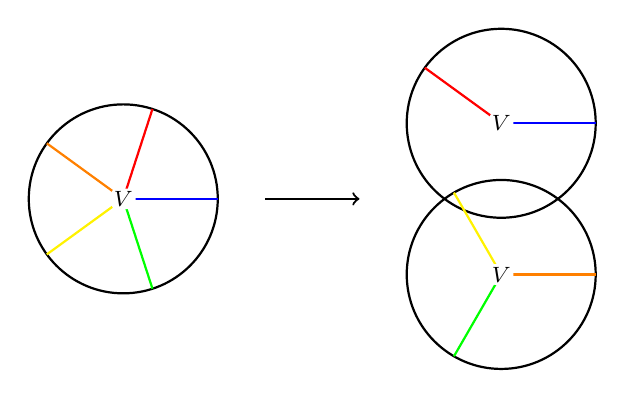
\begin{tikzpicture}[scale=1.2]
  % Left sphere (original) with colored sectors
  \draw[thick] (0,0) circle (1);
  \foreach \angle/\col in {0/blue, 72/red, 144/orange, 216/yellow, 288/green} {
    \draw[thick, \col] (0,0) -- (\angle:1);
  }
  \node[fill=white, inner sep=1pt, rounded corners=2pt] at (0,0) {\footnotesize $V$};

  % Arrow
  \draw[->, thick] (1.5,0) -- (2.5,0);

  % Upper right sphere (reconstructed from 2 parts)
  \begin{scope}[shift={(4,0.8)}]
    \draw[thick] (0,0) circle (1);
    \draw[thick, blue] (0,0) -- (0:1);
    \draw[thick, red] (0,0) -- (144:1);
    \node[fill=white, inner sep=1pt, rounded corners=2pt] at (0,0) {\footnotesize $V$};
  \end{scope}

  % Lower right sphere (reconstructed from 3 parts)
  \begin{scope}[shift={(4,-0.8)}]
    \draw[thick] (0,0) circle (1);
    \draw[thick, orange] (0,0) -- (0:1);
    \draw[thick, yellow] (0,0) -- (120:1);
    \draw[thick, green] (0,0) -- (240:1);
    \node[fill=white, inner sep=1pt, rounded corners=2pt] at (0,0) {\footnotesize $V$};
  \end{scope}
\end{tikzpicture}
\end{center}

Satz in Zermelo-Fraenkel ($\text{ZF}$) + $\text{AC}$ (Auswahlaxiom).
\end{math-stroke}

\begin{spoken-clean}[00:03:50 - 00:06:50]
Ich habe von meinem Kollegen gehört, dass Sie schon die Zermelo-Fraenkel-Axiome behandelt haben. Weiß jemand noch, kennt jemand noch eines? Ein Zermelo-Fraenkel-Axiom?

\inlinemetanote{Ein Student antwortet.}

Das Aussonderungsaxiom, genau. Was sagt das?

\inlinemetanote{Der Student erklärt das Aussonderungsaxiom.}

Ja, genau. Das heißt, man sondert halt all jene Elemente aus, die eine bestimmte Bedingung erfüllen. Und das nullte --- was ist eigentlich das nullte Zermelo-Fraenkel-Axiom?

\inlinemetanote{Ein Student antwortet.}

Genau: Es gibt eine Menge, die keine Elemente enthält. Und dann gibt es halt noch ein paar andere. Und was alle brauchen, die sich täglich nicht mit Logik befassen, sondern mit anderer Mathematik, ist auch das Auswahlaxiom. Das ist quasi das letzte in der Liste --- je nach Zählung ist das dann das zehnte oder so.

Und darum geht es heute. Ich sage es Ihnen jetzt gleich in einem Satz, was es besagt: Wenn Sie eine Menge von nicht-leeren Mengen haben, dann können Sie gleichzeitig aus jeder dieser Mengen ein Element auswählen. Das klingt irgendwie sehr plausibel, nicht sehr kontrovers --- scheint irgendwie nicht so kontrovers zu sein.

Aber aus dem Auswahlaxiom kriegen Sie dann eben zum Beispiel dieses Banach-Tarski-Paradoxon. Sie können dann so eine Kugel aufspalten. Warum heißt das jetzt Paradoxon? Anders gesagt, die Leute, die gesagt haben, es geht nicht mit der Schokolade, warum haben die das so gesehen? Warum denken Sie, es geht nicht? Irgendwie muss es ja einen Grund geben, dass das jetzt ein Paradoxon ist.

Übrigens kommt das Wort aus dem Griechischen: \qt{para} heißt gegen und \qt{doxa} heißt Anschein. Es ist also gegen den Anschein --- es ist eben kein Widerspruch, sondern einfach nur gegen den Anschein. Warum?
\end{spoken-clean}

\begin{student-interaction}[Studentenantwort]
Also man würde erwarten, dass, wenn man das zerschneidet und wieder zusammenfügt, das Volumen gleich bleibt.
\end{student-interaction}

\begin{spoken-clean}[00:06:50 - 00:09:45]
Genau. Wegen des Volumens ist es ein Paradoxon. Der Grund, warum das viele Leute nicht so intuitiv finden, ist das Volumen. Denn wenn alle diese Teile ein wohldefiniertes Volumen hätten, dann ginge es eben nicht --- erst recht, wenn das Volumen auch noch gewisse Eigenschaften erfüllt wie in der Maßtheorie, nämlich Additivität, genauer gesagt endliche Additivität. Andernfalls hätten Sie hier auf der rechten Seite das doppelte Volumen.

Das Lustige ist aber: Diese Teile haben gar kein Volumen. Sie haben zwar ein äußeres Maß, aber kein richtiges Maß. Daher ist das kein Widerspruch, sondern nur ein Paradoxon.

Gut, das wollte ich zum Anfang sagen. Das ist eine Sache, die man aus dem Auswahlaxiom erhält. Das ist jetzt etwas, was wir später nicht direkt verwenden werden; was wir aber verwenden werden, ist eine andere Sache. Ich mache dann gleich alles formal, aber zuerst schreibe ich mal ein bisschen auf, was die Relevanz dieses Auswahlaxioms ist. In der Realität werden Sie Folgendes brauchen, nämlich:
\end{spoken-clean}

\begin{math-stroke}[Äquivalente Aussagen über ZF]
Unter der Annahme der Zermelo-Fraenkel-Axiome ($\text{ZF}$) sind folgende Aussagen äquivalent:
\begin{itemize}
    \item \textbf{AC:} Das Auswahlaxiom (Axiom of Choice)
    \item \textbf{WOP:} Das Wohlordnungsprinzip (Well-Ordering Principle)
    \item \textbf{KZL:} Das Kuratowski-Zornsche Lemma
\end{itemize}
Aus diesen folgt eine fundamentale Aussage der linearen Algebra:
\[
\implies \text{Jeder Vektorraum besitzt eine Basis.}
\]
\end{math-stroke}

\begin{spoken-clean}[00:09:45 - 00:12:15]
Details folgen dann. Wenn man die Zermelo-Fraenkel-Axiome ($\text{ZF}$) annimmt, sind drei Aussagen äquivalent: das Auswahlaxiom, das Wohlordnungsprinzip --- darüber werde ich heute mehr sagen --- und das Kuratowski-Zorn-Lemma.

Dieses Wohlordnungsprinzip besagt: Jede Menge kann wohlgeordnet werden. Was genau eine Wohlordnung ist, werde ich gleich erklären. Man erhält dadurch, dass je zwei Elemente verglichen werden können und jede nicht-leere Teilmenge ein kleinstes Element besitzt.

Und dann gibt es noch das Dritte, was über $\text{ZF}$ äquivalent ist, nämlich das Kuratowski-Zorn-Lemma ($\text{KZL}$). Und das sagt etwas über eine Halbordnung --- das ist jetzt nicht so wichtig, was genau es besagt ---, aber aus diesem Kuratowski-Zorn-Lemma erhalten Sie dann eben, dass zum Beispiel jeder Vektorraum eine Basis besitzt. Und das ist etwas, was Sie in der Realität brauchen werden: Jeder Vektorraum besitzt eine Basis. Vielleicht wird mein Kollege Urech noch etwas dazu sagen, wie man das zeigt, oder es gibt eine Übungsaufgabe dazu --- das gab es bei mir beim letzten Mal, als ich diese Vorlesung gehalten habe.

Dieser Vektorraum ist unendlichdimensional. Wenn er endlichdimensional ist, dann können Sie die Basis konstruieren, haben Sie vielleicht gemacht in der Linearen Algebra mithilfe von Induktion. Aber wenn der Vektorraum unendlichdimensional ist, dann wissen Sie a priori nicht, ob der eine Basis besitzt. Er besitzt sie eben nur wegen des Lemmas von Zorn (bzw. Kuratowski-Zorn), welches äquivalent zum Auswahlaxiom ist. Und das ist für mich im Wesentlichen die Relevanz dieses Auswahlaxioms.

Jetzt habe ich Ihnen hoffentlich einen kleinen Eindruck gegeben, was das ist und wozu es gut ist. Nun werde ich das Ganze genauer ausführen.
\end{spoken-clean}

\section{Das Auswahlaxiom}
\subsection{Formulierung des Auswahlaxioms}

\begin{spoken-clean}[00:12:15 - 00:14:40]
Ich folge jetzt den Notizen, die ich damals geschrieben habe; die sind auch im Internet zu finden --- vielleicht hat das Herr Urech angekündigt, und wenn nicht, können Sie diese in der Pause ja mal suchen. Sie brauchen also nicht alles abzuschreiben, denn es gibt ziemlich ausführliche Notizen dazu. Hoffentlich stimmt die Nummerierung, das kann sich aber natürlich auch mal ändern.

Die Formulierung des Auswahlaxioms ist jetzt Punkt 1.1, auf den ich eingehen möchte: das Auswahlaxiom. Ich werde es jetzt einfach gleich hinschreiben. Das Auswahlaxiom ist die folgende Formel --- dieses Symbol ($\equiv$) bedeutet \qt{ist identisch gleich}. Ich weiß nicht, ob Herr Urech das auch so geschrieben hat.

Es bedeutet Folgendes: Für alle $\mathcal{X}$ --- und ich schreibe jetzt ein geschweiftes $\mathcal{X}$, weil ich mir das als ein Mengensystem denke, das heißt eine Menge von Mengen. Vielleicht haben Sie bei Herrn Urech gehört, dass im Grunde alles eine Menge ist. Wenn Sie eine Menge haben und sich die Elemente davon anschauen, sind das auch wieder Mengen. Mathematisch gesehen ist das also nichts Spezielles, aber ich denke mir das als eine Menge von Mengen, weshalb ich ein geschweiftes $\mathcal{X}$ verwende. Ich nenne das dann auch eine Kollektion von Mengen.

Für jede Kollektion von Mengen, die nicht die leere Menge als Element enthält --- die leere Menge soll also nicht darin liegen ---, gilt, dass es eine Funktion $f$ gibt; diese Funktion heißt dann Auswahlfunktion. Sie muss eine Abbildung von dieser Menge, von dieser Kollektion, zur Vereinigung aller Elemente der Kollektion sein. Das hier ist meine Notation --- nicht nur meine, Herr Urech hat sie vielleicht auch eingeführt --- für die Vereinigung über alle Elemente: $\bigcup \mathcal{X}$. Man vereinigt alle Elemente hier drin. Die Elemente nenne ich jetzt einfach normal große $X$. Ich vereinige also alle Mengen $X$, die in diesem geschweiften $\mathcal{X}$ liegen. Wir haben jetzt eine Abbildung von da nach da.

Das hier ist die Notation für Abbildungen, haben Sie das gesehen? Manchmal schreibt man das $X$ auch dorthin, das ist üblicher, aber ich schreibe es jetzt mal so.

Oh, ja, das ist ein bisschen doof. Jetzt muss ich das noch irgendwie abstellen, das ist immer so eine Sache. Vielleicht einfach drücken, bis alles aus ist... Nein. Entschuldigung. Ja, okay. Hoffentlich kommt's nicht nochmals, vielleicht doch.

\inlinemetanote{Das Mobiltelefon des Dozenten klingelt kurz, er schaltet es stumm.}
\end{spoken-clean}

\begin{math-stroke}[Das Auswahlaxiom]
\begin{equation}
\label{eq:ac}
\text{AC} \equiv \forall \mathcal{X} \left( \emptyset \notin \mathcal{X} \rightarrow \exists f \left( f \in {}^{\displaystyle \mathcal{X}}\!\bigcup \mathcal{X} \land \forall X \in \mathcal{X} \, \bigl( f(X) \in X \bigr) \right) \right)
\end{equation}
Hierbei bezeichnet:
\begin{itemize}
    \item \textbf{$f$:} Eine \newterm{Auswahlfunktion} (Choice function).
    \item \textbf{$\bigcup \mathcal{X}$:} Die Vereinigung des Mengensystems $\mathcal{X}$, definiert als:
    \[
    \bigcup \mathcal{X} := \bigcup_{X \in \mathcal{X}} X = \{ x \mid \exists X \in \mathcal{X} \text{ mit } x \in X \}
    \]
\end{itemize}
\end{math-stroke}

\begin{spoken-clean}[00:14:40 - 00:17:28]
Es gibt also eine solche Auswahlfunktion, die von der ganzen Kollektion von Mengen zur Vereinigung geht, sodass für jedes $X$ in dieser Kollektion gilt: $f(X) \in X$. Darum heißt es eben Auswahlaxiom, und $f$ heißt Auswahlfunktion. Ein solches kleines $f$ wählt aus jedem großen $X$ --- ich mache das normale $X$ mal blau --- ein Element aus. Ich schreibe dafür mal klein $x$. Es wählt ein kleines $x$ aus dieser Menge aus.

Nehmen wir an, Sie haben da ein paar Mengen, vielleicht drei, die einige Elemente enthalten. Jetzt nehme ich diese blaue Menge $X$ hier --- das ist vielleicht die erste --- und wähle ein Element aus; dieses ausgewählte Element ist dann $f(X)$. Das rote Element hier ist $f(X)$, und $X$ ist die blaue Menge. Das mache ich für alle Mengen gleichzeitig. Und dieses Axiom besagt eben, dass es eine solche Auswahlfunktion $f$ gibt. Gut.

Das allgemeinere kartesische Produkt kennt man von zwei Mengen, aber jetzt geht es gerade um unendlich viele Mengen. Da wird es erst richtig interessant. Wenn wir nur endlich viele Mengen betrachten, brauchen wir kein zusätzliches Axiom; dann folgt die Existenz einer solchen Auswahlfunktion $f$ per Induktion.

Man kann es so sehen: Das Auswahlaxiom besagt, dass das kartesische Produkt einer Kollektion von nicht-leeren Mengen ebenfalls nicht leer ist. Die Elemente dieses kartesischen Produkts entsprechen genau solchen Auswahlfunktionen. Das möchte ich jetzt erklären.
\end{spoken-clean}

\begin{math-stroke}[Veranschaulichung der Auswahlfunktion]
\begin{center}
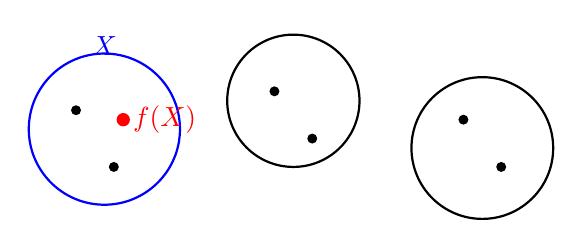
\begin{tikzpicture}[scale=1.2]
  % Three sets (circles)
  \draw[thick, blue] (0,0) circle (0.8) node[above=0.8cm] {$X$};
  \draw[thick] (2,0.3) circle (0.7);
  \draw[thick] (4,-0.2) circle (0.75);
  
  % Elements inside the first set
  \fill[red] (0.2,0.1) circle (2pt) node[right, red] {$f(X)$};
  \fill (0.1,-0.4) circle (1.5pt);
  \fill (-0.3,0.2) circle (1.5pt);
  
  % Elements inside other sets
  \fill (1.8,0.4) circle (1.5pt);
  \fill (2.2,-0.1) circle (1.5pt);
  \fill (3.8,0.1) circle (1.5pt);
  \fill (4.2,-0.4) circle (1.5pt);
\end{tikzpicture}
\end{center}
\end{math-stroke}

\section{Das kartesische Produkt}

\begin{spoken-clean}[00:17:28 - 00:20:25]
Zuerst einmal das Setting. Seien $I$ und ein geschweiftes $\mathcal{X}$ Mengen. Die Menge $I$ denken wir uns als eine Indexmenge. Wir indizieren dann Elemente aus gewissen Mengen mit Indizes aus $I$. Nun haben wir eine Abbildung $X \colon I \to \mathcal{X}$. Sie nimmt einen Index $i \in I$, und wir schreiben $X_i$ für $X(i)$, was eine dieser Mengen sein soll. Man hat also eine Kollektion von Mengen, aber formal gesehen ist das eine Abbildung, die einen Index auf eine Menge abbildet.

Definition des kartesischen Produkts: Ich schreibe dafür ein Kreuz ($\bigtimes$). Letztes Jahr haben die Leute protestiert, dass es hier zu viele Kreuze gibt. Der Grund ist --- schauen Sie, es geht alles irgendwie synchron: Sie haben ein kleines $x \in X$, und das große $X \in \mathcal{X}$. Mir gefällt das irgendwie. Aber wenn es Ihnen nicht gefällt, dürfen Sie die Notation für sich persönlich gerne ändern. Das Kreuz ist ein Kreuz, das möchte ich nicht ändern --- ich mache es jetzt einmal dick. Es steht für das kartesische Produkt.
\end{spoken-clean}

\begin{math-stroke}[Das allgemeine kartesische Produkt]
\textbf{Setting:} Seien $I, \mathcal{X}$ Mengen, $X \colon I \to \mathcal{X}$ eine Abbildung. Wir schreiben:
\[
X_i := X(i) \quad \text{für } i \in I.
\]

\begin{definition}[Allgemeines kartesisches Produkt]\label[definition]{def:cartesian-product}
Das \newterm{kartesische Produkt} der Familie von Mengen $(X_i)_{i \in I}$ ist definiert als:
\begin{equation}
\label{eq:cartesian-product}
\bigtimes X_i = \bigtimes_{i \in I} X_i := \left\{ x \in {}^{I}\!\bigcup \mathcal{X} \;\middle|\; \forall i \in I \colon \underbrace{x_i}_{x(i)} \in X_i \right\}
\end{equation}
\end{definition}
\end{math-stroke}

\begin{spoken-clean}[00:20:25 - 00:22:27]
Ich schreibe jetzt einfach $\bigtimes X$ --- hier steht stillschweigend diese Abbildung $X$ ---, aber man darf das auch so schreiben, wie es an der Tafel steht, dann ist es ein bisschen intuitiver: $\bigtimes_{i \in I} X_i$. Das Erste ist effizient, das Zweite ist intuitiv. Wir haben also das Produkt über alle Indizes $i \in I$ von $X_i$, wobei $X_i$ eine Menge ist. Nehmen Sie zum Beispiel die Indexmenge $I = \{0, 1\}$, dann haben Sie das Produkt $X_0 \times X_1$.

Es ist Folgendes: Man schreibt vielleicht auch ein anderes Produktzeichen, aber ich verwende dieses. Das kartesische Produkt besteht aus allen Funktionen $x$, die einen Index $i \in I$ nehmen und auf ein Element in dieser Vereinigung abbilden, und zwar so, dass für alle $i \in I$ gilt: $x_i$ --- das ist wieder meine Lieblingsnotation für $x(i)$ --- liegt in $X_i$. Anders gesagt: Sie wählen für jeden Index $i$ ein Element aus der entsprechenden Menge $X_i$ aus.
\end{spoken-clean}

\begin{spoken-clean}[00:22:27 - 00:24:41]
Gut, dann könnte ich jetzt hier ein paar Beispiele machen; ich denke aber, Sie sollten sich das selbst anschauen, ich möchte nicht zu viel an die Tafel schreiben. Was ich noch sagen möchte, ist: Wenn Sie nur zwei Mengen $X_0$ und $X_1$ haben und das kartesische Produkt betrachten --- was Sie vermutlich schon gesehen haben, da Sie ja die Zermelo-Fraenkel-Axiome behandelt haben ---, woraus besteht das dann? Was liegt da drin? Das kartesische Produkt zweier Mengen. Ja, bitte?

\inlinemetanote{Ein Student antwortet.}

Paare von Elementen, genau. Ich habe ein Symbol verwendet wie Herr Halbeisen --- haben Sie dieses spitze Klammerpaar $\langle \cdot, \cdot \rangle$ für geordnete Paare auch benutzt? Okay. Dann haben wir hier ein Paar $\langle x_0, x_1 \rangle$, wobei $x_0 \in X_0$ und $x_1 \in X_1$.

Das, was ich jetzt neu eingeführt habe, ist im Grunde genau dasselbe. Genauer gesagt können Sie dieses Paar mit der folgenden Funktion identifizieren: $0 \mapsto x_0$ und $1 \mapsto x_1$. Diese Funktion liegt dann in diesem neuen kartesischen Produkt, wenn Sie die Indexmenge $I = \{0, 1\}$ betrachten.

Das heißt: Das Neue stimmt mit dem Alten überein, wenn Sie nur zwei Mengen haben. Wenn Sie drei Mengen haben, können Sie sich das analog überlegen. Das neue Konzept ist jedoch viel allgemeiner: Wenn Sie unendlich viele Mengen haben --- also wenn die Indexmenge $I$ unendlich ist ---, funktioniert die neue Definition weiterhin, die alte hingegen nicht.

Und jetzt lässt sich die Tafel nicht hochschieben... Jetzt bewegt sich nur die eine Tafel, eben ging es doch noch. Ah, doch.

\inlinemetanote{Der Dozent verschiebt die Tafeln erneut.}
\end{spoken-clean}

\begin{math-stroke}[Spezialfall für zwei Mengen]
Für den Spezialfall $I = \{0, 1\}$ gilt:
\begin{equation}
\label{eq:special-case-two-sets}
X_0 \times X_1 \ni \langle x_0, x_1 \rangle \equiv \begin{pmatrix} 0 \mapsto x_0 \\ 1 \mapsto x_1 \end{pmatrix} \in \bigtimes_{i \in I = \{0, 1\}} X_i
\end{equation}
\end{math-stroke}

\subsection{Umformulierung des Auswahlaxioms}

\begin{spoken-clean}[00:24:41 - 00:27:02]
Und jetzt können wir das Auswahlaxiom eben auch damit formulieren. In meinen Notizen schreibe ich noch ausführlicher dazu, wie diese beiden Formulierungen genau zusammenhängen; das können Sie gerne nachlesen.

Nun kommen wir zur Umformulierung des Auswahlaxioms mithilfe dieses Produkts. Ich schreibe dafür $\text{AC}'$. Das ist die folgende Formel beziehungsweise der folgende Satz: Für alle Indexmengen $I$, für alle Mengensysteme $\mathcal{X}$ und für alle Abbildungen $X \in {}^{I}\!\mathcal{X}$ gilt Folgendes: Wenn für alle Indizes $i \in I$ die Menge $X(i)$ nicht leer ist, dann ist das kartesische Produkt $\bigtimes X$ nicht leer.
\end{spoken-clean}

\begin{math-stroke}[Alternative Formulierung des Auswahlaxioms]
Das Auswahlaxiom lässt sich äquivalent über das allgemeine kartesische Produkt formulieren:
\begin{equation}
\label{eq:ac-prime}
\text{AC}' \equiv \forall I \forall \mathcal{X} \forall X \in {}^{I}\!\mathcal{X} \left( \forall i \in I \, \bigl( X(i) \neq \emptyset \bigr) \rightarrow \bigtimes X \neq \emptyset \right)
\end{equation}

\begin{theorem}[Äquivalenz von AC und AC']\label[theorem]{thm:ac-ac-prime-equivalence}
Unter Annahme der Zermelo-Fraenkel-Axiome ($\text{ZF}$) gilt:
\begin{equation}
\label{eq:ac-equivalence}
\text{AC} \leftrightarrow \text{AC}'
\end{equation}
\end{theorem}
\end{math-stroke}

\begin{spoken-clean}[00:27:02 - 00:28:43]
Das ist die Formulierung, die man in der mathematischen Praxis meistens verwendet: Das kartesische Produkt nicht-leerer Mengen ist nicht leer. Haben Sie dazu Fragen?

Nun möchte ich erklären, wann man das Auswahlaxiom überhaupt benötigt und wann nicht. Wie gesagt: Wenn Sie eine endliche Indexmenge haben, brauchen Sie es nicht; dann können Sie per Induktion zeigen, dass man aus endlich vielen Mengen Elemente auswählen kann. Auch wenn Sie ein eindeutiges Merkmal haben, das aus jeder Menge ein bestimmtes Element auszeichnet, benötigen Sie das Auswahlaxiom nicht. Zum Beispiel, wenn...

Das führt uns zu einer Bemerkung. Betrachten wir eine Abbildung in die Potenzmenge von $\omega$ --- haben Sie dieses Symbol $\mathcal{P}$ für die Potenzmenge, also die menge aller Teilmengen, schon gesehen? ---, sodass jedes $X_i$ nicht leer ist. In diesem Fall benötigen wir kein Auswahlaxiom, um zu zeigen, dass das Produkt aller $X_i$ nicht leer ist. Der Grund dafür ist: Wir wählen $x_i \in X_i$ einfach als das kleinste Element.

Der Punkt ist, dass es hier ein ausgezeichnetes Element gibt, das ein eindeutiges Merkmal besitzt, nämlich das kleinste Element zu sein --- die kleinste natürliche Zahl. Jedes dieser $X_i$ ist eine nicht-leere Teilmenge von $\omega$, also der Menge der natürlichen Zahlen. Die haben Sie auch so bezeichnet, oder? Haben Sie auch $\omega$ geschrieben? Das ist die Menge, deren Existenz durch das Unendlichkeitsaxiom von Zermelo und Fraenkel garantiert wird; sie spielt die Rolle der natürlichen Zahlen $0, 1, 2, \dots$.

In diesem Fall (d.\,h. wenn jedes $X_i \subseteq \omega$ nicht leer ist) nimmt man einfach die jeweils kleinste Zahl. Wir benötigen hier also kein Auswahlaxiom, um eine Auswahl zu treffen. Es gibt eben Situationen, in denen man es nicht braucht.

Eine anschauliche Analogie --- die auf Bertrand Russell zurückgeht --- betrifft Schuhe und Socken. Wenn Sie eine unendliche Kollektion von Schuhpaaren haben, benötigen Sie kein Auswahlaxiom, um aus jedem Paar einen Schuh auszuwählen. Warum? Wie machen Sie das ohne Auswahlaxiom? Ja, bitte?

\inlinemetanote{Ein Student antwortet.}

Genau: Sie nehmen einfach immer den linken Schuh. Dafür brauchen Sie kein Auswahlaxiom, weil es ein eindeutiges Unterscheidungsmerkmal gibt --- der eine Schuh ist links, der andere rechts. Wenn Sie hingegen Socken haben, funktioniert das nicht mehr. Wir nehmen an, dass die beiden Socken eines Paares völlig identisch aussehen. Wenn Sie unendlich viele Sockenpaare haben, können Sie nicht einfach jeweils die linke Socke wählen. In diesem Fall benötigen Sie das Auswahlaxiom. Das illustriert den Unterschied zwischen Schuhen und Socken.
\end{spoken-clean}

\section{Das Wohlordnungsprinzip}
\subsection{Strikte lineare Ordnung und Wohlordnung}

\begin{spoken-clean}[00:28:43 - 00:30:02]
--- das Alte mit diesen Paaren, von mir aus.

Jetzt gibt es die folgende Definition dafür, was eine Wohlordnung ist. Ich nenne die Relation jetzt nicht $R$, sondern verwende das Kleiner-Zeichen ($<$). Und nun erkläre ich zuerst, was eine strikte lineare Ordnung ist, und danach, was eine Wohlordnung ist. Als Erstes haben wir die Bedingung der Trichotomie.

Trichotomie bedeutet: Für alle $x, y \in A$ gilt entweder $x < y$ oder $x = y$ oder $x > y$. Und \qt{entweder} bedeutet hier wirklich \qt{entweder} --- also ein ausschließliches Oder.
\end{spoken-clean}

\begin{spoken-clean}[00:30:02 - 00:30:44]
... und die Trichotomie erfüllt. Übrigens kommt das Wort aus dem Griechischen: \qt{tri} bedeutet drei und \qt{temno} schneiden. Man schneidet die Sache also in drei Teile --- nämlich $x < y$, $x = y$ oder $x > y$ ---, und diese Fälle schließen sich gegenseitig aus. Darum heißt es so.

Als Nächstes: Was bedeutet es noch gleich, dass eine Relation transitiv ist?
\end{spoken-clean}

\begin{student-interaction}[Studentenantwort]
Wenn $x < y$ und $y < z$, dann ist $x < z$.
\end{student-interaction}

\begin{spoken-clean}[00:30:44 - 00:31:13]
Ja, genau: Wenn $x < y$ und $y < z$, dann ist $x < z$.

Transitivität bedeutet also: Für alle $x, y, z \in A$ gilt: Wenn $x < y$ und $y < z$, dann folgt $x < z$. (Übrigens bedeuten meine Pfeile an der Tafel meistens Implikation --- manchmal kann es auch ein Abbildungspfeil sein, aber hier ist es eine Implikation).

Das haben wir jetzt also. Nun kommen wir zur nächsten Definition: Was bedeutet es, ein minimales Element einer Teilmenge zu sein? Sei $S \subseteq A$ eine Teilmenge.
\end{spoken-clean}

\begin{math-stroke}[Strikte lineare Ordnung und Wohlordnung]
\begin{definition}[Strikte lineare Ordnung]\label[definition]{def:strikte-lineare-ordnung}
Sei $<$ eine binäre Relation auf einer Menge $A$, d.\,h. ${<} \subseteq A \times A$.
\begin{enumerate}[label=\textbf{(\roman*)}]
    \item \textbf{Trichotomie:} Für alle $x, y \in A$ gilt entweder $x < y$ oder $x = y$ oder $x > y$.
    \item \textbf{Strikte lineare Ordnung:} $<$ heißt eine \newterm{strikte lineare Ordnung} auf $A$, falls gilt:
    \[
    < \text{ ist transitiv} \quad \land \quad \text{Trichotomie}
    \]
    wobei transitiv bedeutet:
    \[
    \forall x, y, z \in A \colon (x < y \land y < z \rightarrow x < z)
    \]
\end{enumerate}
\end{definition}
\end{math-stroke}

\begin{spoken-clean}[00:31:13 - 00:32:01]
Ein Element $x \in S$ heißt minimal bezüglich unserer Relation $<$, wenn für alle $y \in S$ gilt: $y \not< x$.

Es muss im Allgemeinen nicht so sein, dass ein minimales Element eindeutig ist. Sobald wir eine lineare Ordnung haben, ist das der Fall, aber im Allgemeinen muss das nicht so sein.
\end{spoken-clean}

\begin{math-stroke}
\begin{definition}[Minimales Element]\label[definition]{def:minimales-element}
Sei $S \subseteq A$. Ein Element $x \in S$ heißt \newterm{minimal} bezüglich $<$, falls gilt:
\[
\forall y \in S \colon y \not< x
\]
\end{definition}
\end{math-stroke}

\begin{spoken-clean}[00:32:01 - 00:33:16]
Nun zu Punkt vier: Wohlordnung. Eine Relation $<$ heißt Wohlordnung --- darum geht es heute ja ---, wenn sie all diese Bedingungen erfüllt. Das heißt, sie muss eine (strikte) lineare Ordnung sein --- man kann also je zwei Elemente vergleichen (ich lasse das Wort \qt{strikte} in Zukunft weg) ---, und jede nicht-leere Teilmenge muss ein minimales Element besitzen.
\end{spoken-clean}

\begin{math-stroke}
\begin{definition}[Wohlordnung]\label[definition]{def:wohlordnung}
Eine Relation $<$ heißt eine \newterm{Wohlordnung} auf $A$, falls $<$ eine (strikte) lineare Ordnung ist und jede nicht-leere Teilmenge $S \subseteq A$ ein minimales Element besitzt:
\[
\forall S \subseteq A \ \bigl( S \neq \emptyset \rightarrow \exists x \in S \ \forall y \in S \colon y \not< x \bigr)
\]
\end{definition}
\end{math-stroke}

\begin{spoken-clean}[00:33:16 - 00:34:28]
Das ist die Definition einer Wohlordnung, und um diese geht es heute.

Das Wohlordnungsprinzip ($\text{WOP}$) hat den Status eines Axioms --- nicht eines Theorems, sondern eines Axioms. Es besagt: Auf jeder Menge $A$ existiert eine Wohlordnung.

Ich möchte nun erklären, weshalb das Wohlordnungsprinzip äquivalent zum Auswahlaxiom ist. Das ist das Hauptziel der heutigen Vorlesung. Es gibt ein Theorem, das besagt, dass das Wohlordnungsprinzip und das Auswahlaxiom über $\text{ZF}$ äquivalent sind --- unter der Annahme der Zermelo-Fraenkel-Axiome kann man also das eine aus dem anderen herleiten.
\end{spoken-clean}

\begin{math-stroke}[Das Wohlordnungsprinzip]
\begin{definition}[Wohlordnungsprinzip -- WOP]\label[definition]{def:wop}
Auf jeder Menge $A$ existiert eine Wohlordnung.
\end{definition}
\end{math-stroke}

\begin{math-stroke}[Äquivalenz von AC und WOP]
\begin{theorem}\label[theorem]{thm:ac-wop-equivalence}
Unter Annahme der Zermelo-Fraenkel-Axiome ($\text{ZF}$) gilt:
\[
\text{ZF} \vdash \text{AC} \leftrightarrow \text{WOP}
\]
\end{theorem}
\end{math-stroke}

\begin{proof}[Beweis des Theorems \ref{thm:ac-wop-equivalence}]
\subsubsection{Richtung: Wohlordnungsprinzip impliziert Auswahlaxiom}

\begin{spoken-clean}[00:34:28 - 00:36:58]
Die eine Richtung ($\text{WOP} \implies \text{AC}$) is ziemlich einfach zu beweisen. Ich habe das Wort \qt{Theorem} an der Tafel mit Großbuchstaben geschrieben, weil es sich um ein metamathematisches Theorem handelt. Herr Urech hat das vielleicht nicht so explizit erwähnt, aber es gibt auch Sätze (Theoreme) im formalen Sinne --- also Formeln ohne freie Variablen, bei denen alle Variablen durch Quantoren gebunden sind. Ein metamathematisches Theorem mit Großbuchstaben besagt hier: In $\text{ZF}$ sind das Auswahlaxiom und das Wohlordnungsprinzip äquivalent. Das ist keine Formel im Sinne der Prädikatenlogik erster Stufe, da das Metazeichen $\vdash$ vorkommt. Weiß jemand noch, was dieses Zeichen ($\vdash$) bedeutet?

Genau: Es bedeutet, dass es einen formalen Beweis dieser Äquivalenz aus den Zermelo-Fraenkel-Axiomen gibt. Diese Aussage selbst ist ein metamathematisches Theorem über die Existenz eines solchen Beweises.

Nun zum Beweis der Implikation $\text{WOP} \implies \text{AC}$. Dass man aus dem Wohlordnungsprinzip das Auswahlaxiom erhält, ist relativ einfach. Ich werde hier keinen rein formalen Beweis führen, da das viel zu kompliziert wäre. Stattdessen nutzen wir den gödelschen Vollständigkeitssatz und argumentieren informell, wie man das in der mathematischen Praxis tut. Wie Sie vielleicht bei Herrn Urech gehört haben, erlaubt uns der Vollständigkeitssatz, \qt{normal} zu argumentieren. Wir nehmen also an, das Wohlordnungsprinzip gilt, und zeigen, dass daraus das Auswahlaxiom folgt.
\end{spoken-clean}

\begin{math-stroke}[Beweis der Implikation WOP $\implies$ AC]
\textbf{Annahme:} Das Wohlordnungsprinzip (WOP) gilt. Zeige, dass das Auswahlaxiom ($\text{AC}$) gilt.
\end{math-stroke}

\begin{spoken-clean}[00:36:58 - 00:38:08]
Erinnern wir uns an das Auswahlaxiom: Wir starten mit einem Mengensystem $\mathcal{X}$, das die leere Menge nicht als Element enthält ($\emptyset \notin \mathcal{X}$), und wollen zeigen, dass eine Auswahlfunktion existiert. Sei also $\mathcal{X}$ eine Menge von nicht-leeren Mengen.

Nun wollen wir eine Auswahlfunktion definieren. Dazu nutzen wir den Trick, den ich vorhin erwähnt habe: Wenn wir in jeder Menge $X \in \mathcal{X}$ ein eindeutig ausgezeichnetes Element bestimmen können, sind wir fertig. Dieses ausgezeichnete Element wird das jeweils kleinste Element bezüglich einer Wohlordnung sein.

Das funktioniert wie folgt: Nach dem Wohlordnungsprinzip existiert eine Wohlordnung $<$ auf der Vereinigung aller Mengen in unserem System, also auf $\bigcup \mathcal{X}$.
\end{spoken-clean}

\begin{math-stroke}[Wohlordnung auf der Vereinigung]
Sei $\mathcal{X}$ eine Menge von nicht-leeren Mengen (d.\,h. $\emptyset \notin \mathcal{X}$).
Wegen des Wohlordnungsprinzips (WOP) existiert eine Wohlordnung $<$ auf der Vereinigung:
\[
\bigcup \mathcal{X} = \bigcup_{X \in \mathcal{X}} X
\]
\end{math-stroke}

\begin{spoken-clean}[00:38:08 - 00:39:33]
Wir definieren unsere Auswahlfunktion $f \colon \mathcal{X} \to \bigcup \mathcal{X}$ wie folgt: Für jede Menge $X \in \mathcal{X}$ sei $f(X)$ definiert als das $<$-minimale Element von $X$.

Dieses minimale Element ist eindeutig bestimmt, da wir eine Wohlordnung haben und somit je zwei Elemente vergleichbar sind --- das folgt aus der Trichotomie. Das \qt{entweder} bedeutet hier wirklich ein ausschließliches Oder: Es kann nicht sein, dass $a < b$ und gleichzeitig $b < a$ gilt.

Da jede Menge $X \in \mathcal{X}$ nach Voraussetzung nicht leer ist, existiert in jeder dieser Mengen ein solches minimales Element. Haben Sie dazu Fragen?

Damit haben wir eine wohldefinierte Auswahlfunktion konstruiert und somit das Auswahlaxiom aus dem Wohlordnungsprinzip hergeleitet.
\end{spoken-clean}

\begin{math-stroke}[Konstruktion der Auswahlfunktion]
Wir definieren die Auswahlfunktion:
\[
f \colon \mathcal{X} \to \bigcup \mathcal{X}
\]
durch:
\[
f(X) := \text{das $<$-minimale Element von } X \quad \text{für jedes } X \in \mathcal{X}.
\]
Dieses minimale Element existiert, da $X \neq \emptyset$ and $X \subseteq \bigcup \mathcal{X}$ wohlgeordnet ist. Es ist eindeutig bestimmt aufgrund der Trichotomie der linearen Ordnung $<$.

Somit ist $f$ eine wohldefinierte Auswahlfunktion, und das Auswahlaxiom ($\text{AC}$) ist bewiesen.
\end{math-stroke}
\end{proof}

\section{Ordinalzahlen}
\subsection{Einführung und Definitionen}

\begin{spoken-clean}[00:39:33 - 00:41:28]
Damit gilt das Auswahlaxiom ($\text{AC}$ --- Axiom of Choice).

Diese Richtung ist also bewiesen. Die umgekehrte Implikation ($\text{AC} \implies \text{WOP}$) ist deutlich schwieriger; dafür benötigen wir das Konzept der Ordinalzahlen, was an sich ein sehr interessantes Thema ist.

Ordinalzahlen verallgemeinern die natürlichen Zahlen. Die intuitive Idee ist, dass Ordinalzahlen die Position in einer wohlgeordneten Liste angeben. Jede natürliche Zahl ist eine Ordinalzahl. Ich schreibe das mal auf.

Jede natürliche Zahl $n \in \omega$ (wobei $\omega$ die Menge der natürlichen Zahlen ist) ist eine Ordinalzahl. Im Zermelo-Fraenkel-System ist jede natürliche Zahl definiert als die Menge ihrer Vorgänger: Die Zahl $0$ ist als leere Menge $\emptyset$ definiert, $1$ ist die Menge $\{0\}$, $2$ ist $\{0, 1\}$, und allgemein ist $n = \{0, 1, \dots, n-1\}$. Das sind alles Ordinalzahlen, was man leicht nachprüfen kann. Betrachten wir beispielsweise die Zahl $2 = \{0, 1\}$ und ihr Element $1 = \{0\}$: Dieses Element ist gleichzeitig eine Teilmenge von $2$, da $0 \in 2$ gilt.

Die Idee ist, dass dies eine Position in einer Liste angibt, und das hört bei den endlichen Zahlen nicht auf: Auch $\omega$ selbst ist eine Ordinalzahl.
\end{spoken-clean}

\begin{math-stroke}[Natürliche Zahlen als Ordinalzahlen]
\begin{remark}[Natürliche Zahlen]\label[remark]{rem:natural-numbers}
Jede natürliche Zahl $n \in \omega$ ist eine Ordinalzahl. Dabei ist jede natürliche Zahl definiert als die Menge ihrer Vorgänger:
\begin{align*}
0 &:= \emptyset \\
1 &:= \{0\} = \{\emptyset\} \\
2 &:= \{0, 1\} = \{\emptyset, \{\emptyset\}\} \\
&\;\vdots \\
n &:= \{0, 1, \dots, n-1\}
\end{align*}
\end{remark}
\end{math-stroke}

\begin{spoken-clean}[00:41:28 - 00:42:58]
Dass $\omega$ transitiv ist, ist leicht zu sehen: Wenn Sie ein Element $n \in \omega$ betrachten (das entspricht dem $\beta$ in der Definition, während $\alpha = \omega$ ist), dann sind alle Elemente von $n$ ebenfalls natürliche Zahlen, also gilt $n \subseteq \omega$.

Zudem existiert in jeder nicht-leere Teilmenge von $\omega$ ein kleinstes Element --- das folgt im Wesentlichen aus dem Induktionsprinzip.

Es hört bei $\omega$ aber nicht auf, sondern geht noch viel weiter. Es gibt den Nachfolger $\omega + 1$. Den Nachfolgebegriff haben Sie bereits verwendet, um die natürlichen Zahlen zu definieren --- oft mit dem Symbol $S$ für \emph{successor}. Der Nachfolger von $\omega$ ist definiert als $\omega \cup \{\omega\}$; wir fügen der Menge $\omega$ also einfach $\omega$ selbst als Element hinzu. Das ist ebenfalls eine Ordinalzahl. Insbesondere ist das Element $\omega$ eine Teilmenge von $\omega + 1$, da $\omega \subseteq \omega \cup \{\omega\}$ gilt.
\end{spoken-clean}

\begin{math-stroke}[Formale Definition der Ordinalzahl]
\begin{definition}[Transitivität und Vergleichbarkeit]\label[definition]{def:transitive-set}
Sei $\alpha$ eine Menge.
\begin{enumerate}[label=\textbf{(\roman*)}]
    \item $\alpha$ heißt \newterm{transitiv} $:\iff \forall \beta \in \alpha \ (\beta \subseteq \alpha)$.
    
    Dies ist äquivalent zu: $\forall \beta \in \alpha \ \forall \gamma \in \beta \ (\gamma \in \alpha)$.
    
    \item Zwei Elemente $\beta, \gamma \in \alpha$ heißen \newterm{$\in$-vergleichbar} $:\iff \beta \in \gamma \lor \beta = \gamma \lor \gamma \in \beta$.
\end{enumerate}
\end{definition}

\begin{definition}[Ordinalzahl]\label[definition]{def:ordinal-number}
\begin{enumerate}[label=\textbf{(\roman*)}]
    \setcounter{enumi}{2}
    \item Eine Menge $\alpha$ heißt eine \newterm{Ordinalzahl} $:\iff \alpha$ ist transitiv und bezüglich der Elementrelation $\in$ wohlgeordnet (d.\,h. $\in$-wohlgeordnet).
\end{enumerate}
\end{definition}
\end{math-stroke}

\begin{spoken-clean}[00:42:58 - 00:44:23]
Nach $\omega + 1$ kommt $\omega + 2$, also $S(S(\omega))$, und so weiter. Irgendwann erreichen wir die Grenze $\omega + \omega$. Bei mir in der Vorlesung war das damals eine Übungsaufgabe zu zeigen, dass dies eine wohldefinierte Menge ist. Man muss das natürlich zuerst präzise definieren. Um zu zeigen, dass diese Definition sinnvoll ist beziehungsweise dass diese Menge existiert, benötigt man das Ersetzungsaxiom. Man schreibt diese Menge dann als $\omega \cdot 2$.

Danach folgen $\omega \cdot 3$, $\omega \cdot \omega = \omega^2$, $\omega^3$, $\omega^\omega$ und sogar $\omega^{\omega^\omega}$ --- mit entsprechenden Klammerungen, sodass es mathematisch sehr interessant wird. Wie man diese formal definiert, können Sie im Buch von Herrn Halbeisen nachlesen. Ich werde das hier nicht im Detail ausführen, da wir Ordinalzahlen hier nur als Hilfsmittel benötigen, um zu beweisen, dass aus dem Auswahlaxiom das Wohlordnungsprinzip folgt.
\end{spoken-clean}

\begin{math-stroke}[Die Klasse aller Ordinalzahlen]
Wir definieren die Klasse aller Ordinalzahlen:
\[
\Omega := \{ \alpha \mid \alpha \text{ ist eine Ordinalzahl} \}
\]
\end{math-stroke}

\begin{spoken-clean}[00:44:23 - 00:45:48]
Sie haben bei Herrn Urech gehört, dass es einen wichtigen Unterschied zwischen Klassen und Mengen gibt. Die Klasse aller Ordinalzahlen $\Omega$ ist eine echte Klasse und keine Menge. Das hängt mit dem Burali-Forti-Paradoxon zusammen: Wäre $\Omega$ eine Menge, so wäre sie selbst eine Ordinalzahl und somit ein Element von sich selbst ($\Omega \in \Omega$), was jedoch der Trichotomie widerspricht.

Das Burali-Forti-Paradoxon besagt also, dass die Klasse $\Omega$ keine Menge ist. Damit löst sich dieses Paradoxon auf --- eine echte Klasse ist schlicht \qt{größer} als eine Menge. Haben Sie dazu Fragen?

Cesare Burali-Forti war übrigens eine historische Persönlichkeit. Cesare heißt er, ja. --- Entschuldigung, ich versuche gerade, mein Telefon stummzuschalten, hoffentlich funktioniert es diesmal. Oh, Verzeihung, ich muss herausfinden, wie man das bei diesem Modell macht. Ach, ich hätte einfach... okay, gut, nächstes Mal.
\end{spoken-clean}

\begin{math-stroke}
\begin{theorem}[Burali-Forti-Paradoxon]\label[theorem]{thm:burali-forti}
Die Klasse $\Omega$ aller Ordinalzahlen ist keine Menge.
\end{theorem}
\end{math-stroke}

\subsection{Eigenschaften von Ordinalzahlen}

\begin{spoken-clean}[00:45:48 - 00:47:38]
Vor der Pause habe ich den Begriff der Ordinalzahl eingeführt. Die intuitive Idee ist, dass Ordinalzahlen die Position in einer wohlgeordneten Liste angeben. Jede natürliche Zahl ist eine Ordinalzahl. Ich schreibe das noch einmal an.

Als Bemerkung: Jede natürliche Zahl $n \in \omega$ (wobei $\omega$ die Menge der natürlichen Zahlen ist) ist eine Ordinalzahl. Eine solche natürliche Zahl besteht aus der Menge all ihrer Vorgänger. Die Zahl $0$ ist als leere Menge $\emptyset$ definiert, $1$ ist die Menge $\{0\}$, $2$ ist $\{0, 1\}$, und allgemein ist $n = \{0, 1, \dots, n-1\}$. Das sind alles Ordinalzahlen, was man leicht nachprüfen kann. Betrachten wir beispielsweise die Zahl $2 = \{0, 1\}$ und ihr Element $1 = \{0\}$: Dieses Element ist gleichzeitig eine Teilmenge von $2$, da $0 \in 2$ gilt.

Die Idee ist, dass dies eine Position in einer Liste angibt, und das hört bei den endlichen Zahlen nicht auf: Auch $\omega$ selbst ist eine Ordinalzahl.
\end{spoken-clean}

\begin{math-stroke}
\begin{remark}[Beispiele für Ordinalzahlen]\label[remark]{rem:ordinal-examples}
\begin{enumerate}[label=\textbf{(\roman*)}]
    \item Jede natürliche Zahl $n \in \omega$ ist eine Ordinalzahl.
    \item $\omega$ ist eine Ordinalzahl.
    \item Der Nachfolger von $\omega$, definiert als $\omega + 1 := \omega \cup \{\omega\}$, ist eine Ordinalzahl.
    \item Allgemeiner sind auch $\omega + 2, \dots, \omega \cdot 2, \dots, \omega^2, \dots, \omega^\omega, \dots$ Ordinalzahlen.
\end{enumerate}
\end{remark}
\end{math-stroke}

\begin{spoken-clean}[00:47:38 - 00:49:58]
Dass $\omega$ transitiv ist, ist leicht zu sehen: Wenn Sie ein Element $n \in \omega$ betrachten (das entspricht dem $\beta$ in der Definition, während $\alpha = \omega$ ist), dann sind alle Elemente von $n$ ebenfalls natürliche Zahlen, also gilt $n \subseteq \omega$.

Zudem existiert in jeder nicht-leeren Teilmenge der natürlichen Zahlen ein kleinstes Element --- das folgt im Wesentlichen aus dem Induktionsprinzip.

Es hört bei $\omega$ aber nicht auf, sondern geht noch viel weiter. Es gibt den Nachfolger $\omega + 1$. Den Nachfolgebegriff haben Sie bereits verwendet, um die natürlichen Zahlen zu definieren --- oft mit dem Symbol $S$ für \emph{successor}. Der Nachfolger von $\omega$ ist definiert als $\omega \cup \{\omega\}$; wir fügen der Menge $\omega$ also einfach $\omega$ selbst als Element hinzu. Das ist ebenfalls eine Ordinalzahl. Insbesondere ist das Element $\omega$ eine Teilmenge von $\omega + 1$, da $\omega \subseteq \omega \cup \{\omega\}$ gilt.
\end{spoken-clean}

\begin{math-stroke}[Satz über die Struktur von \texorpdfstring{$\Omega$}{Omega}]
\begin{theorem}\label[theorem]{thm:omega-properties}
Unter Annahme der Zermelo-Fraenkel-Axiome ($\text{ZF}$) gilt:
\begin{enumerate}[label=\textbf{(\roman*)}]
    \item Für jede Ordinalzahl $\alpha \in \Omega$ gilt:
    \[
    \alpha = \{ \beta \in \Omega \mid \beta < \alpha \}
    \]
    wobei $\beta < \alpha :\iff \beta \in \alpha$.
    
    \item Für alle Ordinalzahlen $\alpha, \beta \in \Omega$ gilt die Trichotomie bezüglich der Elementrelation:
    \[
    \alpha \in \beta \quad \lor \quad \alpha = \beta \quad \lor \quad \beta \in \alpha
    \]
    
    \item Jede nicht-leere Klasse $S \subseteq \Omega$ besitzt ein bezüglich $\in$ minimales Element.
    
    \item Die Klasse $\Omega$ ist transitiv, d.\,h. für jedes $\alpha \in \Omega$ gilt $\alpha \subseteq \Omega$.
\end{enumerate}
\end{theorem}
\end{math-stroke}

\begin{spoken-clean}[00:49:58 - 00:53:23]
Nun kommen wir zu einem wichtigen Hilfssatz. Unser Ziel ist es weiterhin zu zeigen, dass das Auswahlaxiom das Wohlordnungsprinzip impliziert --- unter der Annahme der Zermelo-Fraenkel-Axiome ($\text{ZF}$).

Die eine Richtung ($\text{WOP} \implies \text{AC}$) ist ziemlich einfach zu beweisen. Ich habe das Wort \qt{Theorem} an der Tafel mit Großbuchstaben geschrieben, weil es sich um ein metamathematisches Theorem handelt. Herr Urech hat das vielleicht nicht so explizit erwähnt, aber es gibt auch Sätze (Theoreme) im formalen Sinne --- also Formeln ohne freie Variablen, bei denen alle Variablen durch Quantoren gebunden sind. Ein metamathematisches Theorem mit Großbuchstaben besagt hier: In $\text{ZF}$ sind das Auswahlaxiom und das Wohlordnungsprinzip äquivalent. Das ist keine Formel im Sinne der Prädikatenlogik erster Stufe, da das Metazeichen $\vdash$ vorkommt. Weiß jemand noch, was dieses Zeichen ($\vdash$) bedeutet?

Genau: Es bedeutet, dass es einen formalen Beweis dieser Äquivalenz aus den Zermelo-Fraenkel-Axiomen gibt. Diese Aussage selbst ist ein metamathematisches Theorem über die Existenz eines solchen Beweises. Haben Sie dazu Fragen?
\end{spoken-clean}

\begin{proof}[Beweis des Burali-Forti-Paradoxons (Theorem \ref{thm:burali-forti})]
\begin{math-stroke}[Beweis des Burali-Forti-Paradoxons]
Angenommen, die Klasse $\Omega$ aller Ordinalzahlen ist eine Menge.

Aus den Eigenschaften \textbf{(i)}--\textbf{(iv)} in Theorem \ref{thm:omega-properties} folgt:
\begin{itemize}
    \item Da $\Omega$ transitiv ist (Eigenschaft \textbf{(iv)}), ist die Bedingung \textbf{(i)} der Definition \ref{def:transitive-set} erfüllt.
    \item Da jede Teilmenge von $\Omega$ wohlgeordnet ist bezüglich $\in$ (Eigenschaft \textbf{(iii)}), ist $\Omega$ selbst $\in$-wohlgeordnet.
\end{itemize}
Daraus folgt, dass $\Omega$ eine Ordinalzahl ist, d.\,h.
\[
\Omega \in \Omega
\]
Dies steht jedoch im Widerspruch zur Trichotomie (Eigenschaft \textbf{(ii)} von Theorem \ref{thm:omega-properties}) für $\alpha = \beta = \Omega$, wonach entweder $\Omega \in \Omega$ oder $\Omega = \Omega$ oder $\Omega \in \Omega$ gelten müsste, wobei sich diese Fälle gegenseitig ausschließen.

Somit ist die Annahme falsch, und $\Omega$ ist keine Menge.
\end{math-stroke}
\end{proof}

\begin{proof}[Beweis des Theorems \ref{thm:ac-wop-equivalence} (Fortsetzung)]

\subsubsection{Richtung: Auswahlaxiom impliziert Wohlordnungsprinzip}

\begin{spoken-clean}[00:57:26 - 00:58:40]
Wir wollen zeigen, dass das Auswahlaxiom das Wohlordnungsprinzip über $\text{ZF}$ impliziert. Dazu benötige ich den folgenden Hilfssatz: Unter der Annahme der Zermelo-Fraenkel-Axiome impliziert das Auswahlaxiom, dass es für jede Menge $A$ eine Ordinalzahl gibt, die zu $A$ bijektiv ist.

Das heißt: In $\text{ZF}$ impliziert das Auswahlaxiom, dass für jede Menge $A$ eine Ordinalzahl $\alpha \in \Omega$ und eine Bijektion $\Psi \colon \alpha \to A$ existieren.
\end{spoken-clean}

\begin{math-stroke}[Hilfssatz zur Ordinalzahleinbettung]
\begin{lemma}\label[lemma]{lem:ac-ordinal-embedding}
In Zermelo-Fraenkel ($\text{ZF}$) impliziert das Auswahlaxiom ($\text{AC}$), dass es für jede Menge $A$ eine Ordinalzahl $\alpha \in \Omega$ und eine Bijektion $\Psi \colon \alpha \to A$ gibt.
\end{lemma}
\end{math-stroke}

\begin{spoken-clean}[00:58:40 - 01:00:00]
Dieser Hilfssatz ist der eigentliche Hauptknackpunkt im Beweis der Implikation $\text{AC} \implies \text{WOP}$. Sobald man diesen Hilfssatz zur Verfügung hat, lässt sich der Beweis sehr schnell führen. Ich zeige Ihnen jetzt diesen schnellen Teil.

Zuerst einige Bemerkungen, für die ich einen neuen Begriff definieren muss: den Push-Forward einer Relation unter einer injektiven Abbildung. Seien $X$ und $Y$ Mengen, $R$ eine binäre Relation auf $X$ --- also eine Teilmenge $R \subseteq X \times X$ --- und $u \colon X \to Y$ eine injektive Funktion. (Das Symbol $\hookrightarrow$ an der Tafel bedeutet Injektivität).
\end{spoken-clean}

\begin{math-stroke}
\begin{remark}[Push-Forward einer Relation]\label[remark]{rem:push-forward}
Seien $X, Y$ Mengen, $R$ eine binäre Relation auf $X$ (d.\,h. $R \subseteq X \times X$) und $u \colon X \to Y$ eine injektive Funktion (geschrieben als $u \colon X \hookrightarrow Y$).
Wir definieren den \newterm{Push-Forward} $u_* R$ als die folgende binäre Relation auf dem Bild $u[X]$:
\[
u_* R := \bigl\{ \langle u(x), u(x') \rangle \in u[X] \times u[X] \;\big|\; \langle x, x' \rangle \in R \bigr\}
\]
\end{remark}
\end{math-stroke}

\begin{spoken-clean}[01:00:00 - 01:01:59]
Wir definieren den Push-Forward $u_* R$ auf die einzig natürliche Weise: Wir wollen eine Relation auf $Y$ konstruieren. Dazu betrachten wir alle Paare $\langle u(x), u(x') \rangle$, für die das Paar $\langle x, x' \rangle$ in der Relation $R$ liegt. Das definiert eine binäre Relation auf $Y$, also eine Teilmenge von $Y \times Y$, da sowohl $u(x)$ als auch $u(x')$ in $Y$ liegen.

Als Bemerkung 2 (die vorherige Definition war Bemerkung 1): Wenn $<$ eine Wohlordnung auf $X$ ist und $u$ injektiv, dann ist der Push-Forward $u_* <$ eine Wohlordnung auf dem Bild $u[X] \subseteq Y$.

Ich weiß nicht, welche Notation Herr Urech verwendet, aber ich schreibe hier eckige Klammern ($u[X]$), um das Bild der Menge klar von der Funktionsauswertung an einem einzelnen Punkt zu unterscheiden. Das Bild $u[X]$ ist die Menge aller $u(x)$ mit $x \in X$. Der entscheidende Punkt ist, dass wir durch diesen Push-Forward aus einer Wohlordnung auf der linken Seite wieder eine Wohlordnung auf der rechten Seite erhalten.
\end{spoken-clean}

\begin{math-stroke}[Eigenschaften des Push-Forwards]
\begin{remark}[Wohlordnung unter Push-Forward]\label[remark]{rem:wohlordnung-push-forward}
\begin{enumerate}[label=\textbf{(\roman*)}]
    \item Ist $<$ eine Wohlordnung auf $X$ und $u \colon X \to Y$ injektiv, so ist der Push-Forward $u_* <$ eine Wohlordnung auf dem Bild $u[X] \subseteq Y$, wobei:
    \[
    u[X] := \{ u(x) \in Y \mid x \in X \}
    \]
\end{enumerate}
\end{remark}
\end{math-stroke}

\begin{spoken-clean}[01:01:59 - 01:03:41]
Nun beweisen wir die Implikation $\text{AC} \implies \text{WOP}$. Wir nehmen an, dass das Auswahlaxiom gilt. Nach dem Hilfssatz existiert eine Ordinalzahl $\alpha \in \Omega$ und eine Bijektion $\Psi \colon \alpha \to A$. Während ich die Tafel wische, können Sie sich schon einmal überlegen, wie wir daraus mithilfe der Bemerkungen --- insbesondere Bemerkung 2 --- das Wohlordnungsprinzip erhalten. Dann sind wir mit diesem Teil bereits fertig; das geht sehr schnell, da der eigentliche mathematische Gehalt im Beweis des Hilfssatzes steckt.

Da $\alpha$ eine Ordinalzahl ist, ist die Elementrelation $\in_\alpha$ nach unserem vorherigen Satz eine Wohlordnung auf $\alpha$. Das war die Eigenschaft, die ich vorhin angeschrieben habe.

Nun wenden wir Bemerkung 2 auf die Bijektion $\Psi \colon \alpha \to A$ an. Wir bilden den Push-Forward $\Psi_*(\in_\alpha)$ dieser Wohlordnung unter $\Psi$ und erhalten eine Wohlordnung auf $A$. Damit sind wir fertig: Das beweist, dass das Auswahlaxiom das Wohlordnungsprinzip impliziert.
\end{spoken-clean}

\begin{math-stroke}[Beweis: \texorpdfstring{AC $\implies$ WOP}{AC -> WOP}]
\begin{short-proof}[Beweis von AC $\implies$ WOP]
\textbf{Annahme:} Das Auswahlaxiom ($\text{AC}$) gilt. Zeige, dass das Wohlordnungsprinzip ($\text{WOP}$) gilt.

Sei $A$ eine beliebige Menge. Nach dem \cref{lem:ac-ordinal-embedding} existiert eine Ordinalzahl $\alpha \in \Omega$ und eine Bijektion $\Psi \colon \alpha \to A$.

Da $\alpha$ eine Ordinalzahl ist, ist die Elementrelation $\in_\alpha$ eine Wohlordnung auf $\alpha$.
Da $\Psi \colon \alpha \to A$ insbesondere injektiv ist, folgt nach \cref{rem:wohlordnung-push-forward}:
\[
\Psi_*(\in_\alpha) \text{ ist eine Wohlordnung auf } \Psi[\alpha] = A.
\]
Somit existiert eine Wohlordnung auf $A$, was das Wohlordnungsprinzip ($\text{WOP}$) beweist.
\end{short-proof}
\end{math-stroke}
\end{proof}

\subsection{Beweis des Hilfssatzes \ref{lem:ac-ordinal-embedding}}

\begin{proof}[Beweis des Hilfssatzes \ref{lem:ac-ordinal-embedding}]

\begin{spoken-clean}[01:03:41 - 01:05:16]
Nun zum Beweis des Hilfssatzes. Bevor wir formal werden, möchte ich die intuitive Idee erklären. Wir wollen für jede Menge $A$ eine Ordinalzahl $\alpha$ und eine Bijektion $\Psi \colon \alpha \to A$ finden. Die Idee ist, dass wir die Elemente von $A$ nacheinander aufzählen: Wir wählen ein erstes Element und nennen es das nullte, dann wählen wir ein weiteres, davon verschiedenes Element und nennen es das erste, dann das zweite, und so weiter.

Wenn wir Glück haben und $A$ abzählbar ist, sind wir nach unendlich vielen Schritten fertig. Aber selbst wenn $A$ nicht abzählbar ist und wir nach all den natürlichen Zahlen noch nicht alle Elemente erfasst haben, machen wir einfach im Transfiniten weiter: Nach allen natürlichen Zahlen wählen wir das $\omega$-te Element, danach das $(\omega+1)$-te, das $(\omega+2)$-te, und so weiter. Irgendwann haben wir auf diese Weise alle Elemente von $A$ aufgezählt und der Prozess bricht ab.

Das liefert uns genau die gesuchte Bijektion: $0$ wird auf das nullte Element abgebildet, $1$ auf das erste, $2$ auf das zweite, und allgemein jeder Index auf das entsprechende Element. Das ist der grundlegende Trick.

Formulieren wir das nun präzise. Sei $A$ eine Menge und wir nehmen an, dass das Auswahlaxiom ($\text{AC}$) gilt. Der Fall $A = \emptyset$ ist trivial, daher betrachten wir den interessanten Fall $A \neq \emptyset$. Wir definieren $\mathcal{P}^*(A) := \mathcal{P}(A) \setminus \{\emptyset\}$ als die Potenzmenge von $A$ ohne die leere Menge. Nach dem Auswahlaxiom existiert eine Auswahlfunktion $F$ für dieses Mengensystem.
\end{spoken-clean}

\begin{math-stroke}[Beweis des Hilfssatzes: Setup]
Sei $A$ eine Menge.
\textbf{Annahme:} Das Auswahlaxiom ($\text{AC}$) gilt.

Falls $A = \emptyset$, so ist die Behauptung trivial mit $\alpha = 0 = \emptyset$ und der leeren Abbildung $\Psi = \emptyset$.
Sei also $A \neq \emptyset$. Wir definieren:
\[
\mathcal{P}^*(A) := \mathcal{P}(A) \setminus \{\emptyset\}
\]
Nach dem Auswahlaxiom ($\text{AC}$) existiert eine Auswahlfunktion:
\[
F \colon \mathcal{P}^*(A) \to \bigcup \mathcal{P}^*(A) = A
\]
sodass für alle $B \in \mathcal{P}^*(A)$ gilt: $F(B) \in B$.
\end{math-stroke}

\begin{spoken-clean}[01:05:16 - 01:06:31]
Diese Auswahlfunktion $F \colon \mathcal{P}^*(A) \to A$ wählt aus jeder nicht-leeren Teilmenge von $A$ ein Element aus. (Formal geht die Abbildung in die Vereinigung $\bigcup \mathcal{P}^*(A)$, was hier einfach wieder die Menge $A$ ist).

Nun definiere ich den Begriff einer $F$-Menge. Ich weiß nicht, ob ich diese Bezeichnung besonders mag, aber so steht sie im Lehrbuch von Herrn Halbeisen. Ich persönlich würde es eher eine $F$-Abbildung nennen, aber wir bleiben bei der etablierten Bezeichnung $F$-Menge --- stellen Sie sich darunter einfach eine Abbildung vor.

Eine $F$-Menge ist ein geordnetes Paar $\langle \alpha, w \rangle$, wobei $\alpha \in \Omega$ eine Ordinalzahl und $w \colon \alpha \to A$ eine injektive Funktion ist. Hierbei kommt die Auswahlfunktion $F$ ins Spiel: Für jedes $\gamma \in \alpha$ muss gelten: $w(\gamma) = F(A \setminus w[\gamma])$. Wir betrachten also das Bild $w[\gamma]$ (wieder mit eckigen Klammern geschrieben) und ziehen es von $A$ ab. Die Auswahlfunktion $F$ wählt dann ein Element aus dem Komplement $A \setminus w[\gamma]$ aus. Der Trick ist, dass $w(\gamma)$ somit garantiert nicht im bisherigen Bild $w[\gamma]$ liegt, was die Injektivität sichert.
\end{spoken-clean}

\begin{math-stroke}
\begin{definition}[$F$-Menge]\label[definition]{def:f-menge}
Eine \newterm{$F$-Menge} ist ein geordnetes Paar $\langle \alpha, w \rangle$, wobei $\alpha \in \Omega$ eine Ordinalzahl und $w \colon \alpha \to A$ eine injektive Funktion ist, sodass für alle $\gamma \in \alpha$ gilt:
\begin{equation}\label{eq:f-menge-rekursion}
w(\gamma) = F\bigl( A \setminus w[\gamma] \bigr)
\end{equation}
wobei $w[\gamma] := \{ w(\delta) \mid \delta \in \gamma \}$ das Bild von $\gamma$ unter $w$ bezeichnet.
\end{definition}
\end{math-stroke}

\begin{spoken-clean}[01:06:31 - 01:08:09]
Das sichert genau die gewünschte Injektivität. Der Kern des Beweises ist, dass wir in jedem Schritt mithilfe von $F$ ein neues Element auswählen, das noch nicht im Bild der bisherigen Konstruktion liegt.

Nachdem wir definiert haben, was eine $F$-Menge ist, führen wir ein Argument analog zur transfiniten Induktion. Wir betrachten am Ende die Vereinigung aller $F$-Mengen, um die gewünschte Bijektion zu erhalten.

Dazu definieren wir für Ordinalzahlen $\alpha, \beta \in \Omega$ die Relation $\alpha \le \beta$ genau dann, wenn $\alpha \in \beta$ oder $\alpha = \beta$ gilt.

Seien nun $\langle \alpha, v \rangle$ und $\langle \beta, w \rangle$ zwei $F$-Mengen. Behauptung 1 besagt: Falls $\alpha \le \beta$, dann ist die Einschränkung von $w$ auf $\alpha$ identisch mit $v$ (d.\,h. $w|_\alpha = v$). Mit anderen Worten: $w$ ist eine Fortsetzung beziehungsweise Erweiterung von $v$ auf einen größeren Definitionsbereich $\beta \ge \alpha$.
\end{spoken-clean}

\begin{math-stroke}[Eigenschaften von F-Mengen]
Wir definieren für Ordinalzahlen $\alpha, \beta \in \Omega$:
\[
\alpha \le \beta :\iff \alpha \in \beta \lor \alpha = \beta
\]

\begin{lemma}[Behauptung 1]\label[lemma]{lem:f-menge-extension}
Seien $\langle \alpha, v \rangle$ und $\langle \beta, w \rangle$ zwei $F$-Mengen. Falls $\alpha \le \beta$, dann gilt:
\[
w\big|_\alpha = v
\]
\end{lemma}

\begin{center}
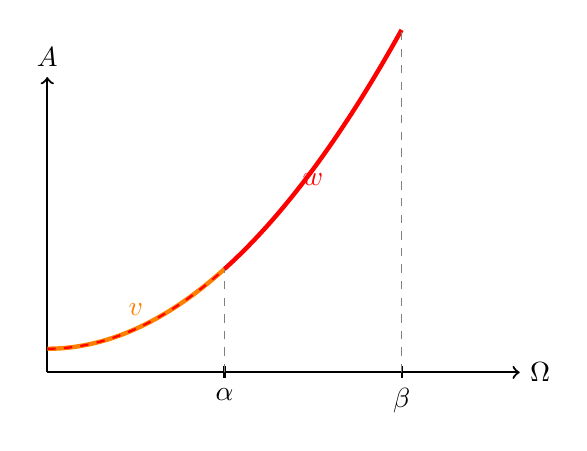
\begin{tikzpicture}[scale=1.5]
    % Axes
    \draw[->, thick] (0,0) -- (4,0) node[right] {$\Omega$};
    \draw[->, thick] (0,0) -- (0,2.5) node[above] {$A$};
    
    % Intervals on axis
    \draw[thick] (1.5,0.05) -- (1.5,-0.05) node[below] {$\alpha$};
    \draw[thick] (3,0.05) -- (3,-0.05) node[below] {$\beta$};
    
    % Orange function v (on \alpha)
    \draw[ultra thick, orange, domain=0:1.5, samples=50] plot (\x, {0.3*\x*\x + 0.2});
    \node[orange, above] at (0.75, 0.4) {$v$};
    
    % Red function w (on \beta, extending v)
    \draw[thick, red, dashed, domain=0:1.5, samples=50] plot (\x, {0.3*\x*\x + 0.2});
    \draw[ultra thick, red, domain=1.5:3, samples=50] plot (\x, {0.3*\x*\x + 0.2});
    \node[red, above] at (2.25, 1.5) {$w$};
    
    % Connecting dashed lines
    \draw[dashed, gray] (1.5,0) -- (1.5,0.875);
    \draw[dashed, gray] (3,0) -- (3,2.9);
\end{tikzpicture}
\end{center}
\end{math-stroke}

\begin{spoken-clean}[01:08:09 - 01:10:21]
Die Funktion wird also fortgesetzt. An der Skizze sieht man: $\beta$ ist das rote Intervall, darauf ist $w$ definiert, und $\alpha$ ist das gelbe Intervall mit der Funktion $v$. Den Beweis von Behauptung 1 lasse ich aus --- das können Sie in den Notizen nachlesen, es ist nicht sehr kompliziert.

Behauptung 2 besagt: Die Klasse $S$ aller $F$-Mengen ist eine Menge. Formal ausgedrückt existiert eine Menge, deren Elemente genau die $F$-Mengen sind. Auch diesen Beweis überspringe ich hier und verweise auf meine Notizen.

Mithilfe dieser beiden Behauptungen beweisen wir nun den Hilfssatz, also die Existenz der Bijektion. Der entscheidende Schritt besteht darin, die Vereinigung über alle $F$-Mengen zu bilden.

Wir definieren $\alpha$ als die Vereinigung aller Ordinalzahlen $\beta$, für die eine Abbildung $w$ existiert, sodass $\langle \beta, w \rangle \in S$ eine $F$-Menge ist. Da $S$ eine Menge ist, ist auch $\alpha$ eine Menge. Analog definieren wir $\Psi$ als die Vereinigung aller Abbildungen $w$ aus den $F$-Mengen in $S$. (In dieser Vorlesung identifizieren wir eine Funktion formal mit ihrem Graphen --- im Gegensatz zu anderen Vorlesungen, wo eine Funktion als Tripel aus Definitionsbereich, Zielbereich und Graph definiert wird. $\Psi$ ist hier also einfach die Vereinigung der Graphen aller dieser Funktionen).

Damit haben wir diese beiden Objekte definiert. Behauptung 3 besagt nun, dass $\Psi$ eine wohldefinierte, bijektive Abbildung von $\alpha$ nach $A$ ist. Das war bei mir damals eine Übungsaufgabe, daher werde ich den Beweis hier nicht vorführen. Es geht mir vor allem darum, dass Sie die tragende Idee des Beweises verstehen.
\end{spoken-clean}

\begin{math-stroke}[Die Menge aller F-Mengen]
\begin{lemma}[Behauptung 2]\label[lemma]{lem:f-mengen-set}
Die Klasse aller $F$-Mengen ist eine Menge:
\[
S := \bigl\{ \langle \beta, w \rangle \;\big|\; \langle \beta, w \rangle \text{ ist eine } F\text{-Menge} \bigr\}
\]
\end{lemma}

Wir definieren die Vereinigung der $F$-Mengen:
\begin{align}
\alpha &:= \bigcup \bigl\{ \beta \in \Omega \;\big|\; \exists w \colon \langle \beta, w \rangle \in S \bigr\} \label{eq:union-ordinals} \\
\Psi &:= \bigcup \bigl\{ w \;\big|\; \exists \beta \colon \langle \beta, w \rangle \in S \bigr\} \label{eq:union-graphs}
\end{align}
\end{math-stroke}

\begin{spoken-clean}[01:10:21 - 01:12:15]
Behauptung 3 besteht aus drei Teilen: Erstens ist $\Psi$ eine wohldefinierte Abbildung von $\alpha$ nach $A$. Dass beim Vereinigen der Graphen kein Widerspruch auftritt, folgt direkt aus Behauptung 1: Da für zwei $F$-Mengen die eine Funktion eine Fortsetzung der anderen ist, stimmen sie auf dem gemeinsamen Definitionsbereich überein. Die Vereinigung der Graphen liefert also wieder einen funktionalen Graphen.

Zweitens ist $\Psi$ injektiv. Das folgt unmittelbar aus der Injektivität der einzelnen Funktionen $w$ der $F$-Mengen.

Drittens ist $\Psi$ surjektiv. Das ist der entscheidende Teil: Durch die Vereinigung aller $F$-Mengen schöpfen wir die gesamte Menge $A$ aus.

Damit erhalten wir eine Bijektion zwischen der Menge $A$ und der Menge $\alpha$. Wir müssen noch sicherstellen, dass $\alpha$ tatsächlich eine Ordinalzahl ist. Das hätte ich eigentlich früher erwähnen sollen: Da $\alpha$ die Vereinigung einer Menge von Ordinalzahlen ist, folgt nach Theorem \ref{thm:omega-properties} (iv), dass $\alpha$ selbst eine Ordinalzahl ist.

Damit ist der Hilfssatz bewiesen --- modulo der Beweise der einzelnen Behauptungen, die ich Ihnen heute nicht im Detail zumuten möchte. Haben Sie dazu Fragen? Es war jetzt vielleicht alles ein bisschen schnell. Ja, bitte?
\end{spoken-clean}

\begin{student-interaction}[Studentenfrage]
Ich wollte fragen, warum bei Beweis Hilfssatz steht \qt{$A$ Menge, Annahme AC gilt}?
\end{student-interaction}

\begin{spoken-clean}[01:12:15 - 01:12:36]
Annahme, genau: Ich nehme das Auswahlaxiom an. Und am Ende erhalte ich die Bijektion zwischen der Ordinalzahl $\alpha$ und der Menge $A$. Dass $\alpha$ eine Ordinalzahl ist, folgt --- wie gesagt --- aus Theorem \ref{thm:omega-properties} (iv), da es sich um eine Vereinigung von Ordinalzahlen handelt. Damit ist der Hilfssatz bewiesen, modulo der Beweise der Behauptungen, die ich Ihnen heute ersparen möchte. Haben Sie dazu noch Fragen? Es war jetzt vielleicht alles ein bisschen schnell.
\end{spoken-clean}

\begin{math-stroke}[Behauptung 3 und Bijektivität]
\begin{lemma}[Behauptung 3]\label[lemma]{lem:f-menge-union-properties}
Seien $\alpha$ und $\Psi$ wie in \eqref{eq:union-ordinals} und \eqref{eq:union-graphs} definiert. Dann gilt:
\begin{enumerate}[label=\textbf{(\roman*)}]
    \item $\Psi$ ist eine wohldefinierte Funktion $\Psi \colon \alpha \to A$.
    \item $\Psi$ ist injektiv.
    \item $\Psi$ ist surjektiv (d.\,h. $\Psi[\alpha] = A$).
\end{enumerate}
\end{lemma}

Da $\alpha = \bigcup \{ \beta \mid \exists w \colon \langle \beta, w \rangle \in S \}$ eine Vereinigung einer Menge von Ordinalzahlen ist, folgt nach \cref{thm:omega-properties} (iv), dass $\alpha$ selbst eine Ordinalzahl ist ($\alpha \in \Omega$).

Da $\Psi \colon \alpha \to A$ nach Behauptung 3 eine Bijektion ist, existiert eine Bijektion zwischen einer Ordinalzahl $\alpha$ und der Menge $A$. Dies beweist den Hilfssatz.
\end{math-stroke}
\end{proof}

\section{Das Kuratowski-Zornsche Lemma}

\begin{spoken-clean}[01:12:36 - 01:14:54]
Als Nächstes möchte ich das Kuratowski-Zorn-Lemma erklären. Ich habe ja versprochen zu zeigen, dass das Auswahlaxiom, das Wohlordnungsprinzip und das Kuratowski-Zorn-Lemma äquivalent sind. Das Kuratowski-Zorn-Lemma ist die Formulierung des Auswahlaxioms, der Sie in der mathematischen Praxis am häufigsten begegnen werden. Dabei geht es um halbgeordnete Mengen. Wir betrachten eine Halbordnung im schwachen Sinne (d.\,h. mit $\le$ statt $<$). Die Axiome dafür sind Reflexivität, Transitivität und Antisymmetrie (d.\,h. $x \le y \land y \le x \implies x = y$).

Wenn auf einer solchen halbgeordneten Menge jede Kette --- das ist eine linear geordnete Teilmenge --- eine obere Schranke besitzt, dann garantiert das Lemma von Zorn die Existenz eines maximalen Elements. Ein solches maximales Element liefert Ihnen dann beispielsweise die Basis eines unendlichdimensionalen Vektorraums.

Das Kuratowski-Zorn-Lemma hat den Status eines Axioms; das Wort \qt{Lemma} ist also historisch bedingt und sollte in Anführungszeichen verstanden werden. Definieren wir zunächst präzise eine Halbordnung: Eine schwache (nicht-strikte) Halbordnung auf einer Menge $P$ ist eine binäre Relation $\le$ auf $P$ mit den folgenden Eigenschaften: Erstens Reflexivität, also $x \le x$ für alle $x \in P$. Zweitens Antisymmetrie: Für alle $x, y \in P$ gilt: Wenn $x \le y$ und $y \le x$, dann folgt $x = y$. Drittens Transitivität. Das Paar $\langle P, \le \rangle$ nennen wir dann eine halbgeordnete Menge.

Eine Kette in $P$ ist eine Teilmenge, die bezüglich $\le$ linear geordnet ist --- in der man also je zwei Elemente vergleichen kann. Eine obere Schranke für eine Teilmenge $S \subseteq P$ ist ein Element $x \in P$, sodass für alle $y$ in dieser Teilmenge gilt: $y \le x$.

Ein Element $x \in P$ heißt maximal, wenn für alle $y \in P$ gilt: Falls $y \ge x$, dann folgt $y = x$. Das bedeutet, dass kein echtes größeres Element existiert. Es bedeutet jedoch nicht, dass dieses maximale Element größer-gleich jedem anderen Element der Menge sein muss --- das ist ein wichtiger Unterschied zu einem größten Element, der bei Halbordnungen eine zentrale Rolle spielt.

Nun kann ich das Kuratowski-Zorn-Lemma ($\text{KZL}$) formulieren: Sei $\langle P, \le \rangle$ eine nicht-leere halbgeordnete Menge, sodass für jede Kette $C \subseteq P$ eine obere Schranke in $P$ existiert. Dann besitzt $P$ mindestens ein maximales Element.
\end{spoken-clean}

\begin{math-stroke}[Halbordnungen und grundlegende Begriffe]
\begin{definition}[Halbordnung]\label[definition]{def:partial-order}
Eine (schwache) \newterm{Halbordnung} (oder partielle Ordnung) auf einer Menge $P$ ist eine binäre Relation $\le$ auf $P$ (d.\,h. ${\le} \subseteq P \times P$), die für alle $x, y, z \in P$ die folgenden Eigenschaften erfüllt:
\begin{enumerate}[label=\textbf{(\alph*)}]
    \item \textbf{Reflexivität:} $x \le x$.
    \item \textbf{Antisymmetrie:} $x \le y \land y \le x \rightarrow x = y$.
    \item \textbf{Transitivität:} $x \le y \land y \le z \rightarrow x \le z$.
\end{enumerate}
Das Paar $\langle P, \le \rangle$ heißt dann eine \newterm{halbgeordnete Menge} (poset).
\end{definition}

\begin{definition}[Kette, Schranke und maximales Element]\label[definition]{def:poset-concepts}
Sei $\langle P, \le \rangle$ eine halbgeordnete Menge.
\begin{enumerate}[label=\textbf{(\roman*)}]
    \item Eine Teilmenge $C \subseteq P$ heißt eine \newterm{Kette} in $P$, falls $C$ bezüglich $\le$ linear geordnet ist, d.\,h.:
    \[
    \forall x, y \in C \colon (x \le y \lor y \le x)
    \]
    \item Ein Element $x \in P$ heißt eine \newterm{obere Schranke} für eine Teilmenge $S \subseteq P$, falls gilt:
    \[
    \forall y \in S \colon y \le x
    \]
    \item Ein Element $x \in P$ heißt ein \newterm{maximales Element} von $P$, falls gilt:
    \[
    \forall y \in P \colon (x \le y \rightarrow x = y)
    \]
\end{enumerate}
\end{definition}
\end{math-stroke}

\begin{nice-box}[Kuratowski-Zornsches Lemma]
\begin{theorem}[Kuratowski-Zornsches Lemma -- KZL]\label[theorem]{thm:zorns-lemma}
Sei $\langle P, \le \rangle$ eine nichtleere halbgeordnete Menge. Falls jede Kette $C \subseteq P$ eine obere Schranke in $P$ besitzt, dann hat $P$ mindestens ein maximales Element.
\end{theorem}
\end{nice-box}

\section{Äquivalenzsätze und historische Einordnung}

\begin{spoken-clean}[01:14:54 - 01:22:06]
Und jetzt gilt das folgende Theorem: In $\text{ZF}$ sind das Auswahlaxiom, das Wohlordnungsprinzip und das Kuratowski-Zorn-Lemma äquivalent. Dass die ersten beiden äquivalent sind, habe ich vorhin bewiesen. Es bliebe noch zu zeigen, dass das Auswahlaxiom und das Lemma von Zorn äquivalent sind. Damit werde ich heute jedoch nicht mehr anfangen, da ich mir die entsprechenden Notizen nicht ausgedruckt habe --- ich dachte nicht, dass ich so schnell durchkommen würde.

Ich möchte stattdessen noch etwas zum historischen Hintergrund des Auswahlaxioms und des Zornschen Lemmas sagen. Historisch gesehen ist die Bezeichnung \qt{Zornsches Lemma} nicht ganz korrekt, obwohl sie sich etabliert hat. Der Erste, der eine ähnliche Formulierung bewiesen hat, war Salomon Bochner. Danach formulierte Kazimierz Kuratowski eine Variante, und erst danach kam Max Zorn. Zorn war also der Letzte in dieser Reihe, aber das Resultat wird heute fast ausschließlich nach ihm benannt.

Wie ich eingangs erwähnt habe, hat das Auswahlaxiom kontraintuitive Konsequenzen wie das Banach-Tarski-Paradoxon, weshalb es historisch sehr umstritten war. Kurt Gödel bewies jedoch 1938, dass das Auswahlaxiom relativ konsistent zu $\text{ZF}$ ist: Falls $\text{ZF}$ widerspruchsfrei (konsistent) ist, so bleibt es auch unter Hinzunahme des Auswahlaxioms konsistent. Man kann die Verneinung des Auswahlaxioms also nicht aus $\text{ZF}$ beweisen, was damals sehr beruhigend war.

Später, im Jahr 1963, zeigte Paul Cohen, dass das Auswahlaxiom auch unabhängig von $\text{ZF}$ ist: Falls $\text{ZF}$ konsistent ist, kann man das Auswahlaxiom nicht aus $\text{ZF}$ beweisen. Das Auswahlaxiom ist somit unabhängig und unentscheidbar in $\text{ZF}$. Man kann es also als Axiom hinzunehmen oder nicht --- in der modernen mathematischen Praxis wird es fast universell akzeptiert, da man ohne es weite Teile der modernen Mathematik nicht betreiben könnte.
\end{spoken-clean}

\begin{math-stroke}
\begin{theorem}[Äquivalenzsatz über ZF]\label[theorem]{thm:zf-equivalences}
Unter Annahme der Zermelo-Fraenkel-Axiome ($\text{ZF}$) sind die folgenden Aussagen äquivalent:
\begin{enumerate}[label=\textbf{(\arabic*)}]
    \item \textbf{AC} (Auswahlaxiom)
    \item \textbf{WOP} (Wohlordnungsprinzip)
    \item \textbf{KZL} (Kuratowski-Zornsches Lemma)
\end{enumerate}
\end{theorem}
\end{math-stroke}

\begin{didactic-insight}[Historische Einordnung und Unabhängigkeit]
Das Auswahlaxiom ($\text{AC}$) nimmt eine einzigartige Stellung in der modernen Mengenlehre ein:
\begin{itemize}
    \item \textbf{Konsistenz (Kurt Gödel, 1938):} Gödel bewies, dass das Auswahlaxiom relativ konsistent zu $\text{ZF}$ ist. Falls $\text{ZF}$ konsistent ist, so ist auch $\text{ZF} + \text{AC}$ konsistent (d.\,h. $\text{ZF} \not\vdash \neg\text{AC}$).
    \item \textbf{Unabhängigkeit (Paul Cohen, 1963):} Cohen bewies mittels der Forcing-Methode, dass das Auswahlaxiom unabhängig von $\text{ZF}$ ist. Falls $\text{ZF}$ konsistent ist, lässt sich $\text{AC}$ nicht aus $\text{ZF}$ beweisen (d.\,h. $\text{ZF} \not\vdash \text{AC}$).
\end{itemize}
Zusammenfassend ist $\text{AC}$ unabhängig und unentscheidbar in $\text{ZF}$. In der mathematischen Praxis wird $\text{AC}$ (bzw. das äquivalente $\text{KZL}$) fast universell akzeptiert, da fundamentale Sätze (wie die Existenz einer Basis in jedem Vektorraum oder der Satz von Tychonoff) ohne dieses Axiom nicht bewiesen werden können.
\end{didactic-insight}

\begin{spoken-clean}[01:22:06 - 01:25:26]
Es gibt dazu eine nette Anekdote des amerikanischen Mathematikers Jerry Bona über das Auswahlaxiom, das Wohlordnungsprinzip und das Lemma von Zorn: \qt{The Axiom of Choice is obviously true, the well-ordering theorem is obviously false, and who can tell about Zorn's lemma?} Und das drückt ein bisschen diese Kontroverse aus, die es mal vor 100 Jahren gab, und heute nicht mehr.

Es war auch noch so --- es gibt noch eine andere Anekdote ---, und zwar geht es da um einen Satz von Tarski. Tarski versuchte, eine äquivalente Formel beziehungsweise Folgendes in einer Zeitschrift einzureichen, nämlich: Dass man aus dem Auswahlaxiom zeigen kann, dass es für jede unendliche Menge $A$ eine Bijektion zwischen der Menge und dem kartesischen Produkt $A \times A$ gibt.

Und dann hat er anscheinend einem Kollegen folgende Geschichte erzählt: Er hat versucht, das bei den \emph{Comptes Rendus de l'Académie des Sciences de Paris} einzureichen --- halt einer Fachzeitschrift. Herr Fréchet war damals zuständig, das zu beurteilen, und Herr Lebesgue auch --- zwei berühmte Mathematiker. Fréchet hat geschrieben, dass eine Implikation zwischen zwei bekannten Sätzen kein neues Resultat sei. Und Lebesgue schrieb, dass eine Implikation zwischen zwei falschen Aussagen nicht interessant sei. Daraufhin hat Herr Tarski aufgegeben und es später nicht mehr bei den \emph{Comptes Rendus} eingereicht.
\end{spoken-clean}

\begin{didactic-insight}[Anekdoten zum Auswahlaxiom]
\textbf{Jerry Bona über die drei Äquivalente:}
\begin{quote}
\qt{The Axiom of Choice is obviously true, the well-ordering theorem is obviously false, and who can tell about Zorn's lemma?}
\end{quote}
Diese berühmte Anekdote illustriert die psychologische Wahrnehmung der drei mathematisch äquivalenten Aussagen: Während das Auswahlaxiom intuitiv selbstverständlich erscheint, wirkt das Wohlordnungsprinzip (wonach z.\,B. auch die reellen Zahlen $\mathbb{R}$ wohlgeordnet werden können, ohne dass man eine solche Wohlordnung explizit angeben kann) völlig kontraintuitiv. Das Lemma von Zorn hingegen ist so komplex formuliert, dass sich jegliche unmittelbare Intuition entzieht.
\end{didactic-insight}

\begin{math-stroke}
\begin{theorem}[Satz von Tarski]\label[theorem]{thm:tarski-cardinal-product}
Für jede unendliche Menge $A$ existiert eine Bijektion zwischen $A$ und dem kartesischen Produkt $A \times A$:
\[
|A| = |A \times A|
\]
\end{theorem}
\end{math-stroke}

\begin{spoken-clean}[01:25:26 - 01:33:02]
Damals war das also eine kontroverse Geschichte --- das ganze Auswahlaxiom und eben diese Umformulierung davon ---, heute jedoch nicht mehr. Es gibt heute wahrscheinlich keinen Mathematiker und keine Mathematikerin mehr, die das Auswahlaxiom strikt ablehnen. Man kann natürlich in der Mathematik seine Axiome frei wählen, aber der Konsens ist: Man nimmt das Auswahlaxiom mit dazu, einfach weil man damit erst gewisse interessante Mathematik betreiben kann. Und das ist auch alles, was man braucht --- Sie brauchen kein neues Axiom mehr.

Modulo vielleicht der algebraischen Geometrie; die machen noch irgendetwas mit einem zusätzlichen Axiom, aber anscheinend kann man das auch wieder loswerden. Es macht die Theorie zwar schöner, aber man kann auch ohne gut leben. Ich glaube, man kann mit dem Auswahlaxiom die gesamte Mathematik betreiben, die Sie so machen möchten --- es sei denn, Sie wollen Logiker oder Logikerin werden, dann machen Sie natürlich etwas anderes und betrachten alle möglichen Axiomensysteme. Aber ansonsten reicht es völlig aus, Zermelo-Fraenkel und das Auswahlaxiom zu haben.

Und jetzt habe ich alles erzählt, was ich wollte. Haben Sie noch Fragen? Gut, dann höre ich jetzt hier auf. Sie können gerne auch nachher noch zu mir kommen und Fragen stellen.
\end{spoken-clean}

\begin{nice-box}[Zusammenfassung der Schlüsselkonzepte]
In dieser Vorlesung haben wir die tiefen Verbindungen zwischen dem Auswahlaxiom und anderen fundamentalen Prinzipien der Mengenlehre kennengelernt:
\begin{itemize}
    \item \textbf{Das Auswahlaxiom ($\text{AC}$):} Garantiert die Existenz einer Auswahlfunktion für jedes System nicht-leerer Mengen. Äquivalent dazu ist die Aussage, dass das allgemeine kartesische Produkt nicht-leerer Mengen nicht leer ist ($\text{AC}'$).
    \item \textbf{Das Banach-Tarski-Paradoxon:} Zeigt, dass eine Kugel in fünf Teile zerlegt und zu zwei identischen Kugeln zusammengesetzt werden kann. Dies ist kein logischer Widerspruch, sondern ein Paradoxon, da die Teilstücke nicht messbar sind (kein wohldefiniertes Volumen besitzen).
    \item \textbf{Das Wohlordnungsprinzip ($\text{WOP}$):} Besagt, dass jede Menge wohlgeordnet werden kann. Wir haben gezeigt, dass $\text{WOP} \implies \text{AC}$ (mittels der minimalen Elemente bezüglich der Wohlordnung) und $\text{AC} \implies \text{WOP}$ (mittels transfiniter Aufzählung über Ordinalzahlen und $F$-Mengen) über $\text{ZF}$ äquivalent sind.
    \item \textbf{Ordinalzahlen ($\Omega$):} Verallgemeinern die natürlichen Zahlen ins Transfinite und dienen als Standardrepräsentanten für Wohlordnungen. Die Klasse aller Ordinalzahlen $\Omega$ ist nach dem Burali-Forti-Paradoxon eine echte Klasse und keine Menge.
    \item \textbf{Das Kuratowski-Zornsche Lemma ($\text{KZL}$):} Garantiert die Existenz maximaler Elemente in halbgeordneten Mengen, in denen jede Kette eine obere Schranke besitzt. Es ist das meistgenutzte Äquivalent des Auswahlaxioms in der Algebra und Analysis (z.\,B. für den Beweis der Existenz einer Basis in jedem Vektorraum).
\end{itemize}
\end{nice-box}

% [SYSTEM] Refinement complete